\documentclass{book}

\usepackage{listings}
\usepackage{theorem}
\usepackage{graphicx}
\usepackage{hyperref}
\usepackage{amsfonts}
\usepackage{amsmath}
\usepackage[table]{xcolor}
\usepackage{array,calc}
\usepackage{amsmath}

\newtheorem{exercise}{Exercise}


\lstset{
  language=Java,
  basicstyle=\ttfamily\footnotesize,
  numbers = left
}

\newcommand{\co}[1]{\lstinline[language=Java, basicstyle=\ttfamily]{#1}}

\begin{document}

\addtocounter{chapter}{3}

\chapter{Point Operations}
A point operation is an image processing step that takes an image as input and that outputs a new image by applying a function to the color of each pixel in the input image. That is, the color of each pixel in the output image depends only on the color of the corresponding pixel in the input image. More formally, each point operation has a corresponding function $f$ that maps colors to colors. The point operation itself applies this function to each pixel:
$$I'(x, y) \leftarrow f(I(x, y))$$
for each position $(x, y)$ in the image. For example, inverting a grayscale image is a point operation with function $f(c) = 255 - c$. Similarly, the identify transform is a point operation with function $f(c) = c$. As we will explain in Section~\ref{sec:contrast-stretching}, the function being applied can depend on the image itself.

In the remainder of this chapter, we will study a number of point operations.

\section{A Tiny Framework for Point Operations}
Each point operation applies a function to each pixel in the image. To model the common aspects shared by all point operations, we define an abstract class \co{PointOperation}. 
\begin{lstlisting}
public abstract class PointOperation {
  public abstract int f(int color);
  
  public void applyTo(ImageProcessor ip) {
    for(int x = 0; x< ip.getWidth(); x++) {
      for(int y = 0; y < ip.getHeight(); y++) {
        ip.putPixel(f(ip.getPixel()));      
      }    
    }
  }
}
\end{lstlisting}
Specific point operations will be modelled by subclasses of \co{PointOperation}. In particular, subclasses should override the abstract method \co{f} with their own function. The method \co{applyTo} modifies the given \co{ImageProcessor} by applying \co{f} to each pixel. Let's look at an example. Inverting a grayscale image is a point operation with function $f(c) = 255 - c$. We can represent inversion by defining a subclass of \co{PointOperation} that overrides \co{f}. 
\begin{lstlisting}
public class Gray8Invert extends PointOperation {
  @Override  
  public int f(int color) {
    return 255 - color;
  }
}
\end{lstlisting}
A grayscale image can be inverted as follows:
\begin{lstlisting}
ImageProcessor ip = ...
Gray8Invert invertor = new Gray8Invert();
invertor.applyTo(ip);
\end{lstlisting}
We can visualize the function corresponding to a point operation in a plot. For example, the plot corresponding to grayscale inversion is the following:
\begin{center}
\includegraphics[scale=0.15]{inversion-plot.png} % todo: better plot
\end{center}

\begin{exercise}
Thresholding is a point operation that converts a grayscale image to a binary image by mapping dark pixels to black and light pixels to white. The function for thresholding is the following:
$$threshold(c) = \left\{\begin{array}{c l}
  0 & \text{if $c \leq 127$}\\
  1 & \text{otherwise}\\
\end{array}
\right.$$
Draw the plot corresponding to thresholding and implement thresholding by defining a new subclass \co{Gray8Threshold} of \co{PointOperation}. Thresholding \co{lena-gray.png} results in the following image:
\begin{center}
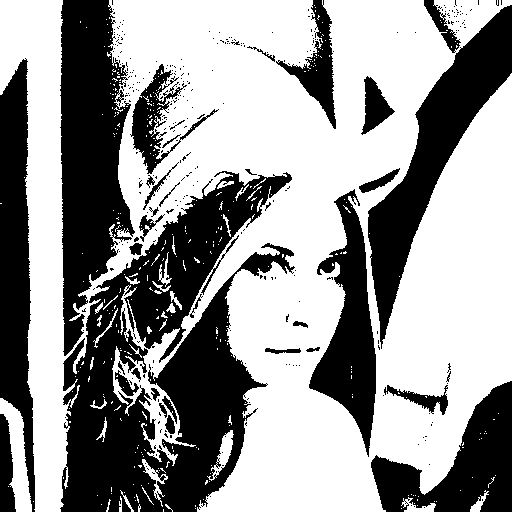
\includegraphics[scale=0.10]{lena-binary.png}
\end{center}
\end{exercise}

\begin{exercise}
Modify \co{Gray8Threshold} such that the bound (\co{127}) is no longer fixed. More specifically, add a constructor that takes the bound as an argument. Thresholding \co{lena-gray.png} with bound 180 results in the following image:
\begin{center}
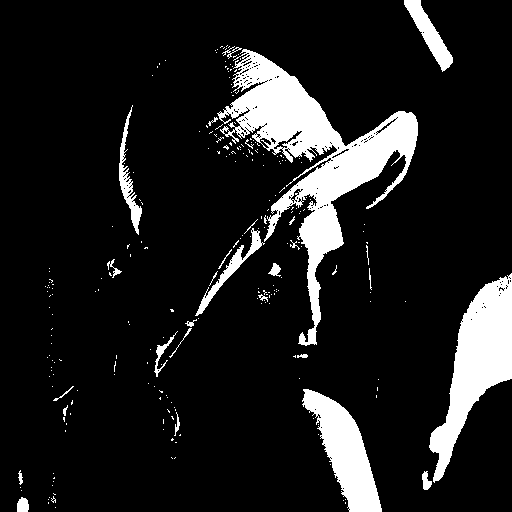
\includegraphics[scale=0.10]{lena-binary-bound-180.png}
\end{center}
\end{exercise}

\begin{exercise}
Thresholding reduces the number of colors in the image to two, black and white. Posterization is a generalization of thresholding to multiple colors. For example, when posterizing a grayscale image to three colors, the range 0 to 85 is mapped to 0, 86 to 170 is mapped to 128 and finally colors in the  range 171 to 255 are mapped to 255. Thus, the function for 3-color posterization is the folllowing:
 $$posterize3(c) = \left\{\begin{array}{c l}
  0 & \text{if $0 \leq c \leq 85$}\\
  128 & \text{if $86 \leq c \leq 170$}\\
  255 & \text{if $171 \leq c \leq 255$}\\
\end{array}
\right.$$
The plot corresponding to this function looks as follows:
\begin{center}
%\includegraphics[scale=0.10]{posterize3-plot.png} % todo
\end{center}
Implement a point operation \co{Gray8Posterize} to posterize grayscale images. The desired number of colors should be a parameter of the class' constructor. Posterizing \co{lena-gray.png} to 4 colors results in the following image:
\begin{center}
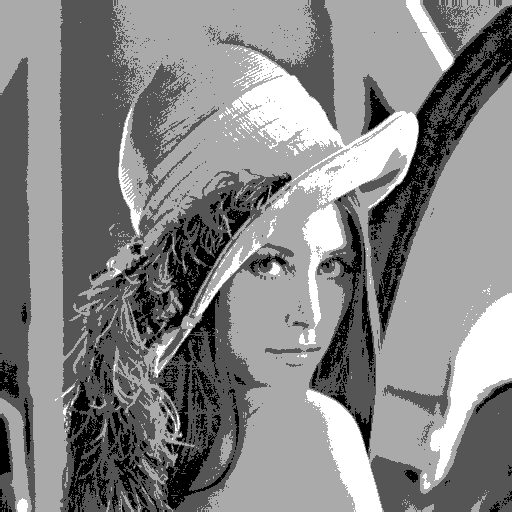
\includegraphics[scale=0.20]{lena-gray-posterized4.png}
\end{center}
\end{exercise}

\begin{exercise}\label{ex:desaturate}
Many graphics editing programs provide a way to \emph{desaturate} an RGB color image. For example, in Gimp this option is available via the menu item \texttt{Colors>Desaturate...}. Desaturation converts all colors in an RGB color image to corresponding shades of gray. After desaturation, the three color components are equal in each pixel (i.e. $R=G=B$).

In Gimp, the conversion of an RGB color to a shade of grade is either based on lightness, luminosity or the channel average. 
\begin{center}
\includegraphics[scale=0.4]{desaturate-gimp.png}
\end{center}
The three functions corresponding to these different conversions are respectively defined as follows:
$$\begin{array}{l}
desaturate_{lightness}((r, g, b)) = (x, x, x)\\
\quad \text{where $x = \max(r, g, b) + \min(r, g, b)) / 2$}\\
\\
desaturate_{luminosity}((r, g, b)) = (x, x, x)\\
\quad\text{where $x = 0.21 r + 0.72 g + 0.07 b$}\\
\\
desaturate_{average}((r, g, b)) = (x, x, x)\\
\quad\text{where $x = (r + g + b)/3$}\\
\end{array}$$
The difference between the three kinds of desaturation is shown below (from left to right: lightness, luminosity and average-based):
\begin{center}
\includegraphics[scale=0.20]{lena-desaturated-lightness.png}
\includegraphics[scale=0.20]{lena-desaturated-luminosity.png}
\includegraphics[scale=0.20]{lena-desaturated-average.png}
\end{center}
Implement desaturation:
\begin{itemize}
  \item Define a new enum \co{DesaturationType} with three values: \co{LIGHTNESS}, \co{LUMINOSITY} and \co{AVERAGE}.
  \item Create a new point operation \co{Desaturate}. The constructor of this class has a parameter of type \co{DesaturationType} that allows callers to select the desired kind of desaturation.
\end{itemize}
\end{exercise}

\section{Composing Point Operations}
Multiple point operation can be \emph{composed}. That is, more complex point operations can be constructed by chaining several simple operations. For example, the conversion of an RGB image to sepia can be built by applying the following two point operations:
\begin{enumerate}
  \item Desaturate the image.
  \item Increase the red and green channels and decrease the blue channel of each pixel to make the image more yellow and brown.
\end{enumerate}
More formally, a point operation with function $f$ can be composed with a point operation with function $g$ by first applying $f$ to each pixel and afterwards applying $g$: 
$$I'(x, y) \leftarrow g(f(I(x, y)))$$
We add composition of point operations to our framework by defining a new subclass of \co{PointOperation} called \co{CompositePointOperation}:
\begin{lstlisting}
public class CompositePointOperation extends PointOperation {
  private final PointOperation first;
  private final PointOperation second;
  
  public CompositePointOperation(PointOperation first, PointOperation second) {
    this.first = first;
    this.second = second;  
  }
  
  @Override
  public int f(int color) {
    int tmp = first.f(color);
    return second.f(tmp);  
  }
}
\end{lstlisting}
In addition, we extend the class \co{PointOperation} itself with a new method \co{before}:
\begin{lstlisting}
  public PointOperation before(PointOperation other) {
    return new CompositePointOperation(this, other);
  }
\end{lstlisting}
This method returns a new point operation that chains \co{this} and \co{other}. That is, applying the new point operation corresponds to first applying \co{this} and afterwards applying \co{other}.

\begin{exercise}
Write a program to convert an RGB color image to sepia:
\begin{itemize}
  \item Converting an image to sepia takes two steps: (1) desaturation and (2) brownification. We have already implemented the first step in exercise~\ref{ex:desaturate}. Implement the point operation \co{Brownify} with the following function:
  $$\begin{array}{c}
brownify((r, g, b)) = \\
(r+ 2{depth}, g + {depth}, b - {intensity})\\
\end{array}$$
where  ${depth}$ and ${intensity}$ are parameters of brownification.  Setting ${sepiaDepth}$ to $20$  and ${sepiaIntensity}$ to $30$ produces nice results. 
  \item Conversion to sepia can then be coded as follows:
\begin{lstlisting}
ImageProcessor ip = ...;
Desaturate desaturate = new Desaturate(DesaturationType.AVERAGE);
Brownify brownify = new Brownify(20, 30);
PointOperation convertToSepia = desaturate.before(brownify);
convertToSepia.applyTo(ip);
\end{lstlisting}
The following image was generated from \texttt{lena.png}:
\begin{center}
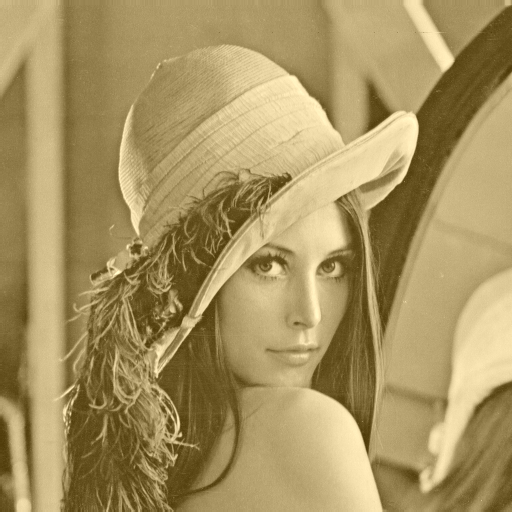
\includegraphics[scale=0.20]{lena-sepia.png}
\end{center}
\end{itemize} 
\end{exercise}
Note that it is also possible to encapsulate conversion to sepia in its own class as follows:
\begin{lstlisting}
public class ConvertToSepia extends CompositePointOperation {
  public ConvertToSepia() {
    super(new Desaturate(DesaturationType.AVERAGE), new Brownify(20, 30));  
  }
}
\end{lstlisting}

\section{Grayscale Contrast Stretching}\label{sec:contrast-stretching}
The contrast of a grayscale image is the difference between the minimum and maximum pixel value occurring in the image. Images with low contrast are often flat, foggy and visually dull. Low contrast color images typically lack vivid colors. For example, the images based on \texttt{lena-gray.png} shown below have decreasing contrast (205, 125 and 45 respectively):
\begin{center}
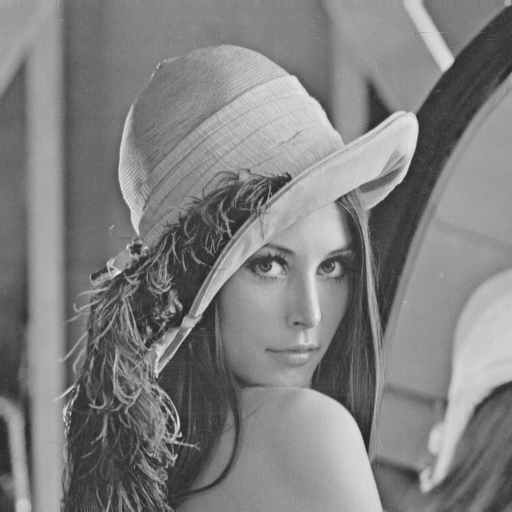
\includegraphics[scale=0.2]{lena-gray.png}
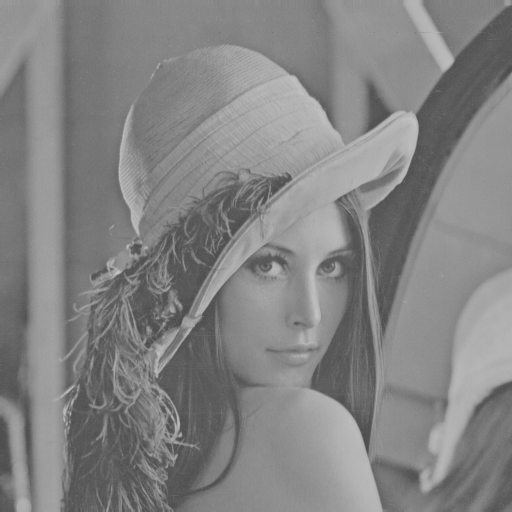
\includegraphics[scale=0.2]{lena-reduced-contrast-125.png}
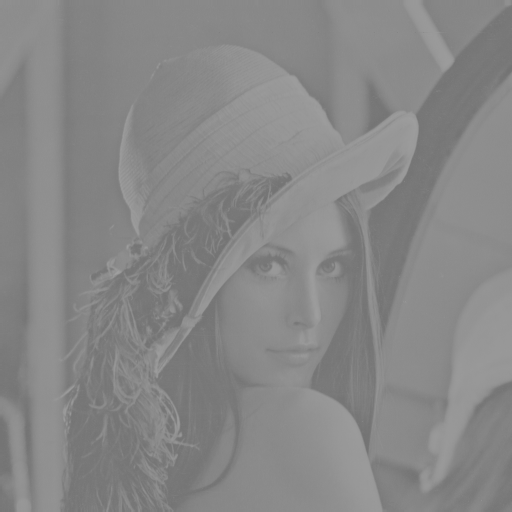
\includegraphics[scale=0.2]{lena-reduced-contrast-45.png}
\end{center}
The histograms of these images are shown below:
\begin{center}
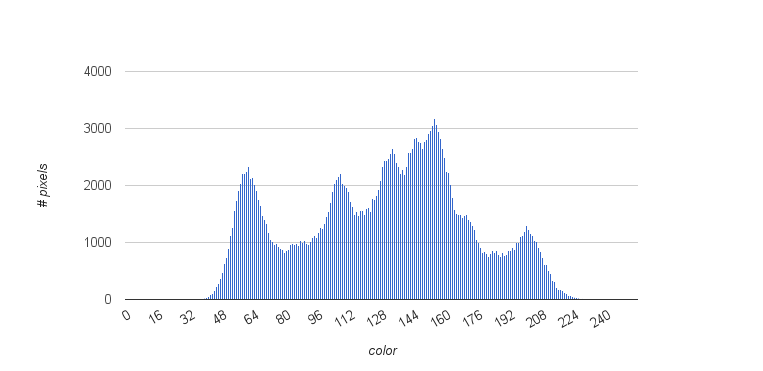
\includegraphics[scale=0.35]{lena-gray-histogram.png}
\includegraphics[scale=0.35]{lena-gray-reduced-contrast-125-histogram.png}
\includegraphics[scale=0.35]{lena-gray-reduced-contrast-45-histogram.png}
\end{center}

Contrast stretching is a point operation that stretches the contrast of an image to the entire available range. The first step in contrast stretching is to compute the minimum and maximum pixel value occurring in the image\footnote{You have already implemented this functionality in the class \co{Gray8Histogram} in the previous chapter.}. Given these boundary values, contrast stretching can be implemented as a composition of two point operations:
\begin{itemize}
  \item Subtract the minimum pixel value from each pixel. That is, apply the following function to each pixel:
$$subtract(c) = c - {min}$$
Subtracting the minimum pixel value moves the entire histogram to the left. For example, applying this operation to \co{lena-gray.png} results in the following histogram:
\begin{center}
\includegraphics[scale=0.35]{lena-gray-subtract-35-histogram.png}
\end{center}
  \item Rescale the pixel values to the entire available range by multiplying them with $255 / (max - min)$. That is, apply the following function to each pixel:
$$multiply(c) = c \frac{255}{max - min}$$
After this multiplication, the histogram spans the entire available available range, i.e. 0 to 255:
\begin{center}
\includegraphics[scale=0.35]{lena-gray-stretched-histogram.png}
\end{center}
\end{itemize}

\begin{exercise}
How does contrast stretching affect the dynamic range of an image?
\end{exercise}

\begin{exercise}
Implement contrast stretching as a composite point operation. Apply this point operation to \texttt{oneinfiniteloop-low-contrast.png}. 
\end{exercise}

\begin{exercise}
Apply your contrast stretcher to \texttt{mysteryperson.png}. Who is this mysterious woman hiding in the fog?
\end{exercise}

\begin{exercise}
Apply your contrast stretcher to \texttt{mysteryperson2.png}. What do you see? Why?
\end{exercise}

\begin{exercise}
\textbf{extra} Given two values \co{low} and \co{high} between 0 and 255, implement a point operation that stretches (or shrinks) the histogram to the interval \co{(low, high)} instead of \co{(0, 255)}. Use this point operation to \emph{reduce} the contrast of \texttt{lena-gray.png}.
\end{exercise}

\subsection*{Improved Grayscale Contrast stretching}
Contrast stretching as described above does not work well if the image contains a few extreme pixel values (e.g. 0 or 255) which are not be representative of the main image content. For example, while the minimum and maximum pixel values in \texttt{mysteryperson2.png} are 0 and 255, most pixels lie in the range 105 to 110. However, contrast stretching does not work well because it amounts to subtracting zero from each pixel and afterwards multiplying by one ($(255 / (255 - 0)$). In other words, contrast stretching has no effect at all on \texttt{mysteryperson2.png}! How can we solve this problem?

The problem caused by extreme pixel values can be avoided by ``ignoring'' (or saturating) a fixed percentage of the pixels in the lower and upper ends of the color range when computing the minimum and maximum pixel value occurring in the image. That is, instead of computing the minimum and maximum pixel value, we compute two limiting values \co{low} and \co{high} such that a fixed percentage of all pixels has value less than or equal to \co{low} and such that a fixed percentage of all pixels has value greater than or equal to \co{high}.  For example, if we ignore 1\% on each side in an image with 10000 pixels, then \co{low} is the smallest color such that there at least 100 pixels in the image with value less than or equal to \co{low}. 

Assuming that the fraction of pixels ignored on each side is $p$, the values of \co{low} and \co{high} for an image with $N$ pixels can easily be computed from the cumulative histogram $H$:
$$\begin{array}{c}
\mathtt{low} = \min \{ c \mid H(i) \geq N.p \} \\
\mathtt{high} = \max \{ c \mid H(i) \leq N.p \} \\
\end{array}$$
Let's look at an example. Suppose we want to compute \co{low} for a 100x100 image with the following cumulative histogram:
$$\begin{array}{rcl}
H(0) & = & 0\\
H(1) & = & 30\\
H(2) & = & 52\\
H(3) & = & 112\\
H(4) & = & 184\\
H(5) & = & 404\\
& \dots &\\
\end{array}$$
If we saturate 1\% on each side, \co{low} is the smallest color that has cumulative histogram value of at least 100 (= 1 percent of 10000). Thus, \co{low} equals $3$.

Given the values of \co{low} and \co{high}, improved contrast stretching can be implemented as a composition of two point operations:
\begin{itemize}
  \item Subtract \co{low} from each pixel. That is, apply the following function to each pixel:
$$subtract(c) = \left\{\begin{array}{c l}
  c - {low} & \text{if ${low} \leq {c}$}\\
  0 & \text{otherwise}\\
\end{array}
\right.$$
  \item Rescale the pixel values to the entire available range by multiplying them with $255 / ({high} - {low})$. That is, apply the following function to each pixel:
$$multiply(c) = \left\{\begin{array}{c l}
  0 & \text{if $c < {low}$}\\
  c \frac{255}{{high} - {low}} & \text{if ${low} \leq c \leq {high}$}\\
  255 & \text{otherwise}\\
\end{array}
\right.$$
\end{itemize}

\begin{exercise}
Implement improved contrast stretching. Apply your improved contrast stretcher to \texttt{mysteryperson2.png}.  Who is this mysterious woman hiding in the fog?
\end{exercise}

Improved contrast stretching is available in practically any image processing software. For example, the auto-contrast operation in Adobe Photoshop saturates 0.5\% of all pixels.

\begin{exercise}
What is the effect of setting the saturation percentage too high? 
\end{exercise}

\begin{exercise}
Write an ImageJ plugin for contrast stretching. Allow the user to select the percentage of pixels that will be saturated on each side via a dialog.
\end{exercise}

\begin{exercise}\textbf{extra}
Add a preview check box to your plugin such that the user can preview the resulting image while selecting the appropriate value for the number of saturated pixels. Chaper 1
%hardref
explains how to add previewing to your plugins.
\end{exercise}

\section{Two-image Point Operations}
A \emph{two-image point operation} is an image processing operation that takes two images as input and that outputs a new image by applying a function to each pixel pair. That is, the value of each pixel in the output image depends only on the colors of the corresponding pixels in both input images. More formally, each two-image point operation has a corresponding function $f$ that maps color pairs to colors. Given two images $I_1$ and $I_2$, the two-image point operation applies this function to each pixel pair:
$$I'(x, y) \leftarrow f(I_1(x, y), I_2(x, y))$$
for each position $(x, y)$ in $I_1$.

To model the common aspects shared by all two-image point operations, we define an abstract class \co{TwoImagePointOperation}. 
\begin{lstlisting}
public abstract class TwoImagePointOperation {
  public abstract int f(int color1, int color2);
  
  public void applyTo(ImageProcessor ip1, ImageProcessor ip2) {
    for(int x = 0; x < ip1.getWidth(); x++) {
      for(int y = 0; y < ip1.getHeight(); y++) {
        int color1 = ip1.getPixel(x, y);
        int color2 = ip2.getPixel(x, y);
        int newcolor = f(color1, color2);
        ip1.putPixel(x, y, newcolor);
      }    
    }
  }
}
\end{lstlisting}
Specific two-image point operations will be modelled as subclasses of the class \co{TwoImagePointOperation}. In particular, subclasses should override the abstract method \co{f} with their own function. The method \co{applyTo} modifies \co{ip1} by applying \co{f} to each pixel pair.

Let's look at an example. Averaging grayscale images is a two-image point operation with function $f(c_1, c_2) = (c_1 + c_2) / 2$. We can represent averaging by defining a subclass of \co{TwoImagePointOperation} that overrides \co{f}. 
\begin{lstlisting}
public class Gray8Average extends TwoImagePointOperation {
  @Override  
  public int f(int color1, int color2) {
    return (c_1 + c_2) / 2;
  }
}
\end{lstlisting}
Two grayscale images can then be averaged as follows:
\begin{lstlisting}
ImageProcessor ip1 = ...
ImageProcessor ip2 = ...
Gray8Average average = new Gray8Average();
average.applyTo(ip1, ip2);
\end{lstlisting}
%The function corresponding to a two-image point operation can be visualized as a 3d surface plot:
%todo

\begin{exercise}
Implement a two-image point operation called \co{Averager} for averaging grayscale images as a subclass of \co{TwoImagePointOperation}. Applying this operation to \texttt{stevejobs-gray.png} and \texttt{billgates-gray.png} results in the following image:
\begin{center}
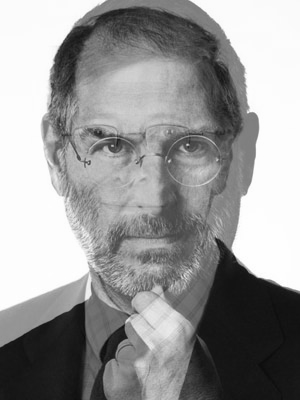
\includegraphics[scale=0.2]{jobs-gates-average.png}
\end{center}
\end{exercise}

\subsection{Chroma Keying}
Chroma keying is a technique to place an object or person in a new scene often used in movies and television productions. The subject is first filmed in front of a green or blue background, and afterwards this background is replaced by a new background. For example, weather man Roby Roels presents the weather in front of a green screen. The viewer however sees the picture shown on the television on the right.
\begin{center}
\includegraphics[scale=0.25]{roby-chromakey.jpg}
\end{center}

\begin{exercise}
The directory \texttt{jasma/dip/pointoperations/student-images} contains a number of images of students in front of a green wall. Select an image from this directory. Try to write a two-image point operation to place the students in front of a new background. That is, replace each pixel in the background image by the corresponding pixel in the foreground image, unless the foreground pixel is ``sufficiently green''.  \texttt{jasma/dip/pointoperations/backgrounds} contains some example backgrounds. You will notice that is hard to find the suitable bounds for the red, green and blue channels that properly isolate the subject.
\end{exercise}

\subsubsection*{HSV}
Isolating a particular color range (e.g. a green background) is hard in the RGB color model. HSV is an alternative to RGB where each color is represented using three components: hue, saturation and value. Hue represents the color, saturation the amount of color and value represent the brightness. Hue always lies between 0 and 360 (representing an angle) and saturation and value both lie between 0 and 1.

\begin{exercise}
Experiment with the HSV color model on

 \href{http://www.cosc.canterbury.ac.nz/mukundan/cogr/HSVColor.html}{http://www.cosc.canterbury.ac.nz/mukundan/cogr/HSVColor.html}. 
 
Adjust the sliders and inspect the resulting colors. What is the HSV triple corresponding to black? What about red and white? How can you create various shades of gray? What happens if you decrease the saturation? What happens if you decrease the value?
\end{exercise}

An RGB triple $(r, g, b)$ can be converted to a HSV triple $(h, s, v)$ as follows:
\begin{itemize}
  \item Normalize the red, green and blue channels to the range 0 to 1 by dividing each channel by 255:
  $$\begin{array}{rcl}
  r_n & = & r / 255;\\
  g_n & = & g / 255;\\
  b_n & = & b / 255;\\
  \end{array}$$
  \item Define ${max}$ as the maximum of $r_n$, $g_n$ and $b_n$. Similarly, define ${min}$ as the minimum of $r_n$, $g_n$ and $b_n$. 
  \item If ${max} = 0$, then the HSV triple is $(0, 0, 0)$.
  \item Otherwise, if $r_n=g_n=b_n$, then the HSV triple is $(0, 0, r_n)$.
  \item Otherwise,
  %
  $$\begin{array}{rcl}
  h & = & \left\{\begin{array}{c l}
  (0 + (g_n - b_n) / ({max} - {min})) \times 60 & \text{if $r_n= {max}$}\\
  (2 + (b_n - r_n) / ({max} - {min})) \times 60 & \text{if $g_n = {max}$}\\
 (4 + (r_n - g_n) / ({max} - {min})) \times 60 & \text{if $b_n = {max}$}\\
\end{array}
\right.\\
  & &\\ 
  s & = & ({max} - {min}) / max\\ 
  & &\\
  v & = & \max(r_n, g_n, b_n)\\
  \end{array}$$
If $h$ is negative, add $360$ to $h$.
\end{itemize}

\begin{exercise}
Write a static method \co{getHSVComponentsFromInt} to convert an integer (that represents a color in the RGB model) to a HSV triple.
\begin{lstlisting}
public static double[] getHSVComponentsFromInt(int color) {
  double[] components = new double[3];
  ...
  components[0] = ...; // hue
  components[1] = ...; // saturation
  components[2] = ...; // value
  return components;
}
\end{lstlisting}
\end{exercise}

\begin{exercise}
The directory \texttt{jasma/dip/pointoperations/student-images} contains a number of images of students in front of a green wall. Select an image from this directory. Write a two-image point operation to place the students in front of a new background. That is, replace each pixel in the background image by the corresponding pixel in the foreground image, unless the foreground pixel is ``sufficiently green''. To determine whether a pixel is ``sufficiently green'', convert it to HSV using \co{getHSVComponentsFromInt} and check whether it is lies within a certain range (in the HSV model).The directory \texttt{jasma/dip/pointoperations/backgrounds} contains some example backgrounds.
\end{exercise}

\subsection{Alpha Blending}
Alpha blending is a two-image point operation that computes the weighted sum of two input images, assigning weight $\alpha$ to the first image and $1 - \alpha$ to the second. Averaging is a special case of alpha blending with $\alpha$ equal to $0.5$.

\begin{exercise}
Implement grayscale alpha blending in a class \co{AlphaBlender}. $\alpha$ is a parameter of the constructor of this class.
\end{exercise}

\begin{exercise}
Extend the class \co{AlphaBlender} such that it can handle both grayscale and RGB color images. For RGB color images, each individual channel is blended separately. For example, blending the RGB triples $(0, 100, 200)$ and $(100, 0, 100)$ with $alpha=0.25$ result in the triple $(75, 25, 125)$.   
\end{exercise}

Alpha blending can be used to fade one image into another by slowly changing the value of $\alpha$. 

\begin{exercise}
Write a (main) method to slowly fade one image into another. Hint: You can force an \co{ImageWindow} to update by calling \co{updateAndDraw} on the corresponding \co{ImagePlus}.
\end{exercise}

\subsection{Spot the Difference}
Consider the two images shown below\footnote{source:\href{http://www.allstarpuzzles.com}{http://www.allstarpuzzles.com}}:
\begin{center}
\includegraphics[scale=0.4]{spotthedifference1.jpg}
\includegraphics[scale=0.4]{spotthedifference2.jpg}
\end{center}
What are the differences between both images? Did you find all 16? Let's write a program to find out.

\begin{exercise}
Write a program that highlights the differences in two RGB color images. Compare the corresponding pixels in each image. If they are equal, decrease the brightness by dividing each color channel by $4$; otherwise, change the color to red. Use your program to find differences in \texttt{spotthedifference1.jpg} and \texttt{spotthedifference2.jpg}.
\end{exercise}

\section{Color Contrast Stretching}\label{sec:color-contrast-stretching}

%\section{Post-it Images}
%\section{LUT}
%misteryimage
% operations from 

\end{document}